% !TEX root = sprints.tex
\noindent \Large{\textbf{Summary}}\\
\normalsize Team Expeditus was able to accomplish most of the objectives for sprint 3.5 and 4. Sprint 3.5 focused mostly on designing a new base plate for the hexrotor and calibrating the flight controller. During this sprint it was agreed on by the team members to set aside work on the simulation as too much time was being consumed by issues encountered. The UAV was able to flown under manual control successfully by the end of Sprint 3.5. Sprint 4 focused on autonomous flight testing, flight control specific message passing in the ROS framework, and reapproach to vision. By the end of the sprint the autonomous flight was successfully tested and a software package for AR tag tracking was successfully compiled and run.\\
\vspace{5mm}
\\
\noindent \Large{\textbf{Team Work}}
\normalsize
\begin{itemize}
\item \textbf{Jonathan Dixon:} Worked on UAV build, AR tracking, and UAV flight.
\item \textbf{Dylan Geyer:} Worked on UAV build, AR tracking, and UAV flight.
\item \textbf{Christopher Smith:} Worked on UAV build, message passing, AR tracking, and UAV flight. 
\item \textbf{Steven Huerta:} Worked on UAV build, AR tracking, and UAV flight. 
\end{itemize}

\vspace{5mm}
\noindent\Large{\textbf{Completed Backlog}}\\
\vspace{2mm}\\
\large{\textbf{Common Development Tasks}}
\normalsize
\begin{itemize}
\item \textbf{Build UAV.}\\
The UAV was assembled before winter break, however, it was apparent that the power distribution board did not fit appropriately, and in addition, the team realized that more room would be needed on the center plate to accommodate the control hardware and sensors. Team members modeled a new plate that was larger and printed the plates. These printed plates will be temporary, as carbon fiber will be used for the final build. The new plates provided the necessary room from the distro board, as well as being able to easily accommodate the flight controller, Odroid, and other sensors.\\
\item \textbf{Test flight under manual control} \\
The UAV was first tested under manual control within the King Center at SDSMT. The manual flight was successful and validated the build. The UAV was responsive to pilot controls.
\item \textbf{Autonomous Flight} \\
The testing of the autonomous flight validated the capability of the flight controller to provide the hexrotor speed controllers the necessary and correct signals, as well as validating the build of the UAV.

This objective is also relevant to the following user stories:
\begin{itemize}
\item \textbf{U-1 As a user, I want to communicate the waypoints to the UAV:} \\
The team successfully sent a series of "missions" to the flight controller including take-off, waypoint navigation goals, and landing. The team used QGroundControl GUI to easily mark points and define the associated action for the UAV.
\item \textbf{O-1 As an owner, I want the UAV to autonomously take-off from the landing pad:} \\
The mission provided to the flight controller instructed the UAV to take-off and achieve a certain height before executing the next mission. The UAV repeatedly executed these instructions according to parameters provided through the GUI mission setup.
\item \textbf{O-2 As an owner, I want the UAV to autonomously navigate through a set of waypoints:} \\
The UAV navigated to the waypoints assigned. This process was repeated for a set of waypoints to ensure that navigation of these points was being successfully handled by the flight controller. The team also observed that despite a flexible frame, caused by the material used in our temporary assembly plates, and some unsecured rotation in one of the rotor arms, the flight controller still successfully navigated through the waypoints.
\item \textbf{O-3 As an owner, I want the UAV to autonomously return to the location of the landing pad:} \\
The UAV navigated back to the location of the landing area designated. Though this was achieved simply by defining the return as the last waypoint mission that the flight controller will execute. It was also observed that if the user uses the landing mission, the flight controller will determine the direct line to land at that point, which is definitely problematic if the landing area is higher than the altitude of the UAV. It causes the UAV to "skip" along the surface. However, this will not be an issue for our team, as we will not be using the landing mission. \\
The navigation is very accurate relative to expectations. The same navigation points used for takeoff were used for the final point of navigation and landing. The flight controller consistently set UAV within two feet of the takeoff point. This has caused the team to re-evaluate the needs for a landing pad. The team feels confident that with the GPS, the flight controller will allow the UAV to navigate to a point where an AR tag alone can be used to provide visual guidance to the UAV.
\end{itemize} 
\end{itemize}


\vspace{5mm}
\noindent\Large{\textbf{Uncompleted Tasks}}\\
\vspace{2mm}\\
\noindent \large{\textbf{Common Development Tasks}}
\normalsize
\begin{itemize}
\item \textbf{Setup Hexrotor Simulation in Gazebo}
The team has decided to indefinitely postpone development of the specific hexrotor simulation. The time invested on resolving software and hardware conflicts was monopolizing project time.
\end{itemize} 

\vspace{3mm}
\noindent \large{\textbf{As an owner, I want the UAV to autonomously land on the landing pad without damaging the craft}}
\normalsize
\begin{itemize}
\item \textbf{Landing Algorithm Simulation}\\
As the team has ceased simulation development, initial testing for the landing algorithm will not occur using the simulation. The proposed method for testing is to review logs generated by our vision guided landing solution while passing the UAV, without props, over the landing AR tag and reviewing the messages passed to the flight controller for descent. The team will specifically test for a controlled landing that will prevent damage to the UAV or the landing pad from the force of impact.
\item \textbf{Modify/Rewrite implementation as necessary}\\
Though not completed, progress was made on modifying our implementation of the landing algorithm to only include the AR tag tracking. The tracking tool (fig.~\ref{fig:artracker}) that we have successfully tested will provide us with distance information necessary to correctly judge the distance from our landing target, as well as calculate a safe rate of descent.
\begin{figure}[h]
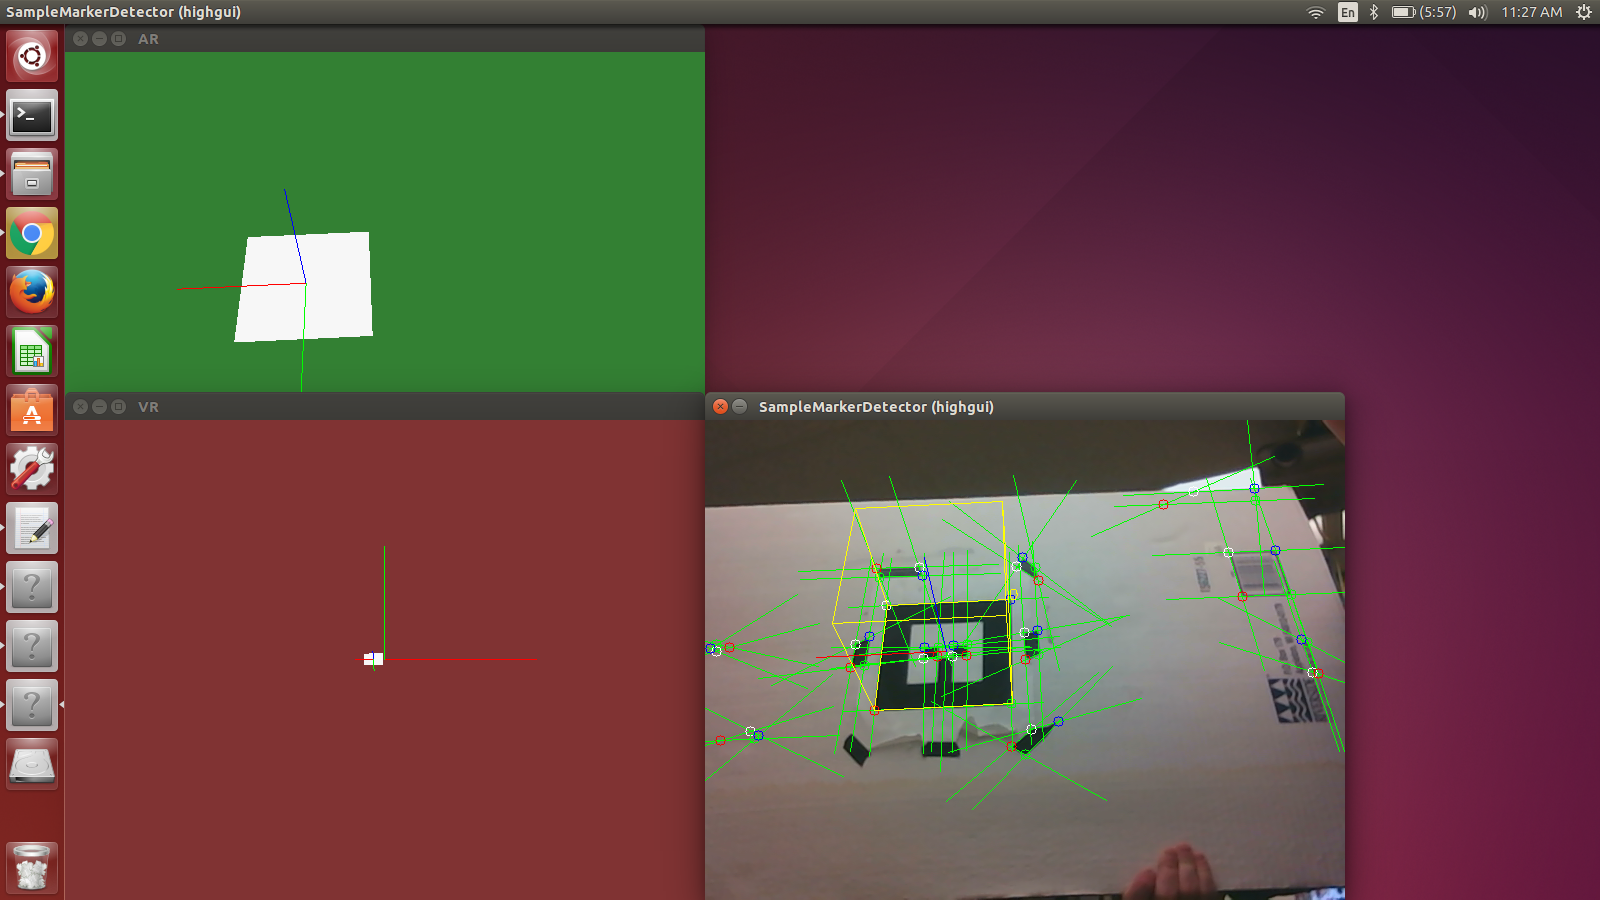
\includegraphics[width=8cm]{images/AlvarExample.png}
\centering
\caption{ALVAR AR Tracker testing with laptop webcam}
\label{fig:artracker}
\end{figure}

\end{itemize}



\vspace{3mm}
\noindent \large{\textbf{As an owner, I want the UAV to autonomously land on the landing pad with the correct orientation.}}
\normalsize
\begin{itemize}
\item \textbf{Landing Algorithm Simulation}\\
As mentioned previously, as our simulation development has ended, our team will utilize the sensors to generate log data to evaluate. The team will specifically test for orientation corrections that will provide the correct alignment on landing.
\item \textbf{Modify/Rewrite implementation as necessary}\\
As mentioned previously, our visual landing approach has changed. We hope to be able to easily modify the existing software to provide information regarding the orientation of the AR tag to use to change the orientation of the UAV as necessary during landing.
\end{itemize}

\vspace{6mm}
\noindent\Large{\textbf{Prototype}}\\
\normalsize
Our prototype for this sprint is mainly just an assembled hexrotor UAV that is able to follow GPS waypoints. Throughout the assembly process, we did small tests to be sure that we were on the right track. At first, we just kept the UAV in the lab and turned to rotors to verify that they were wired correctly and spinning in the right directions. We then had a manual test flight in the gym, where we discovered that the UAV is quite stable and responsive. Finally, we tested the GPS waypoint navigation with a series of flights. We started small, just having the UAV fly to the end of the driveway at first, eventually working our way up to having the UAV take off, move through a series of waypoints, and return to land on the same location it took off from. Over the course of our testing, we estimate that we will be able to trust the GPS to get us above our landing pad. As stated above, this means that we feel confident that we will be able to trust GPS to get us directly above the landing pad. \newline\newline
We have videos of these GPS tests up on \href{https://www.youtube.com/channel/UCfcuqDXKMLgbUWu3rt9rITA}{YouTube}.

